
\section{Zielsetzung}
In diesem Versuch sollen zunächst verschieden periodische elektrische
Schwingungen in ihre Fourier-Komponenten zerlegt werden. Anschließend sollen
ebendiese Funktionen wieder aus ihren theoretisch errechneten Anteilen
zusammengesetzt werden.

\section{Theorie}
Als periodische Funktionen werden jene Funktionen bezeichnet, welche nach
einer bestimmten Periodendauer T oder einer festen Distanz D erneut ihren
ursprünglichen Startwert annehmen, so dass
\begin{align}
  & f(t+T)=f(t) \\
  \text{und \quad}      & f(x+D)=f(x)
  \label{eqn:period}
\end{align}
gilt. Häufig auftretende Funktion sind hierbei Sinus- und Cosinusfunktion,
welche durch eine bestimmte Amplitude $a_n$ bzw. $b_n$ und eine Periodendauer T
charakterisiert sind.
Das Fouriersche Theorem besagt zudem, dass ein Großteil der stetigen periodischen
Funktionen aus der Summation mehrer dieser Funktion zusammensetzen lässt gemäß
der Gleichung
\begin{equation}
   f(t)= \frac{1}{2}a_0 + \sum_{n=1}^\infty \left(a_n \cos n \frac{2 \pi}{T}t
   + b_n \sin n \frac{2 \pi}{T}t\right)
\end{equation}
wobei die Reihe gleichmäßig konvergent ist. Die entsprechenden Amplituden
berechnen sich durch
\begin{align}
  & a_n = \frac{2}{T} \int_0^T f(t) \cos n \frac{2 \pi}{T}t dt \\
  \text{und \quad}     & b_n = \frac{2}{T} \int_0^T f(t) \sin n \frac{2 \pi}
  {T}t dt
\end{align}
mit n $\in \symbb{N} $. Es treten dabei nur ganzzahlige Vielfache der
Grundfrequenz $\nu = \frac{1}{T} $ auf, welche auch als harmonische Oberwellen
bezeichnet werden. Trägt man diese gegen ihre jeweilige Amplitude auf, ergibt
sich daraus ein diskretes Linienspektrum, wie es in Abbildung
\ref{fig:spektrum} zu sehen ist.
\begin{figure}[H]
  \centering
  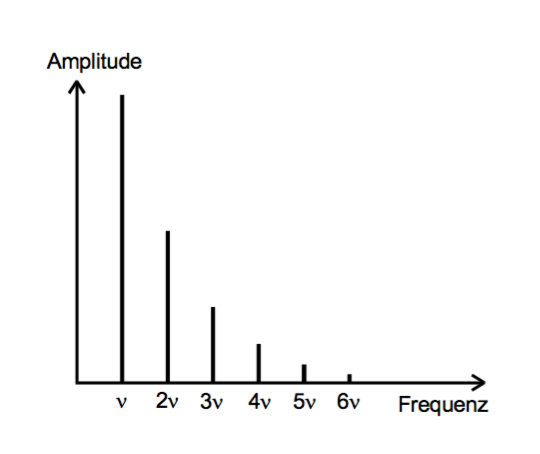
\includegraphics[height=7cm]{Spektrum.png}
  \caption{Linienspektrum einer Fourier-Ananlyse \cite{skript}}
  \label{fig:spektrum}
\end{figure}
Handelt es sich bei der zu approximiernden Funktion f(t) nicht um eine
stetige Funktion, so kommt es zu endlichen Abweichungen der Reihe,
was auch als Gibbssches Phänomen bezeichnet wird. \\
Soll hingegen eine nicht periodische zeitliche Funktion in ihr
Frequenzspektrum zerlegt werden wird statt der Fourier-Reihe die
Fourier-Transformation der Form
\begin{equation}
  g(v) = \int_{-\infty}^{\infty} f(t)e^{i\nu t} dt
\end{equation}
verwendet. Hierbei ergeben periodische Vorgänge erneut in Spektrum aus
$\delta$-Funktionen und nicht periodische Funktionen transformieren sich zu
kontinuirlichen
Spektren. Da es jedoch in der Praxis nicht möglich ist über einen unendlichen
Zeitraum zu integrieren kommt es zu Abweichungen in Form von Linien endlicher
Breite statt $\delta$-Funktionen und Nebenmaxima.
